\section{Part III - Multivariable control}\label{sec:part3}
\subsection{Problem 1 - State-Space Representation}
We put the system in a state-space formulation on the form:
\begin{gather*}
    \mathbf{\dot{x}} = \mathbf{Ax} + \mathbf{Bu}
\end{gather*}
where A and B are matrices, and our state and input vector are: 
\begin{gather*}
    \mathbf{x} = 
    \begin{bmatrix}
        \tilde{p}\\\dot{\tilde{p}}\\\dot{\tilde{e}}
        \end{bmatrix}
     \text{  and  } \mathbf{u} = 
    \begin{bmatrix} \tilde{V_s}\\\tilde{V_d} \end{bmatrix}
\end{gather*}
This gives us the following state-space model:
\begin{gather*}
     \begin{bmatrix}
        \dot{\tilde{p}}\\\ddot{\tilde{p}}\\\ddot{\tilde{e}}
    \end{bmatrix}
    \text{ = } \begin{bmatrix}
        0 & 1 & 0 \\
        0 & 0 & 0 \\
        0 & 0 & 0 \\ \end{bmatrix}
    \begin{bmatrix}
         \tilde{p}\\\dot{\tilde{p}}\\\dot{\tilde{e}}
    \end{bmatrix}
    \text{ + } \begin{bmatrix}
        0 & 0 \\
        0 & K_1 \\
        K_2 & 0 \\
    \end{bmatrix}
    \begin{bmatrix} \tilde{V_s}\\\tilde{V_d} \end{bmatrix}
\end{gather*}

\subsection{Problem 2 - Linear Quadratic Regulator}
We now aim to track the reference $\mathbf{r}
= \begin{bmatrix} \tilde{p_c,} & \tilde{\dot{e_c}}
\end{bmatrix}^T$ for the pitch angle $\tilde{p}$ and elevation rate $\dot{\tilde{e}}$. The reference values $\tilde{p}_c$ and $\dot{\tilde{e}}_c$ are given by the joystick, the x-axis and y-axis respectively. Firstly, we examine if the system is controllable. The controllability matrix is given by:
\begin{gather*}
    \mathcal{C} = 
    \begin{bmatrix} \mathbf{B} & \mathbf{AB} &
    \mathbf{A^2B} \end{bmatrix}
    = \begin{bmatrix}
    0 & 0 & 0 & K_1 & 0 & 0 \\
    0 & K_1 & 0 & 0 & 0 & 0 \\
    K_2 & 0 & 0 & 0 & 0 & 0
    \end{bmatrix}
\end{gather*}
We see that $\mathcal{C}$ has full rank, which means that the system is controllable. In order to actually control the system, we implement a controller of the form:
\begin{gather*}
    \mathbf{u} = \mathbf{Pr} - \mathbf{Kx}
\end{gather*}
In the controller, $\mathbf{r}$ is the reference given by the joystick output. The matrix $\mathbf{K}$ corresponds to the linear quadratic regulator (LQR) for which the control input $\mathbf{u} = -\mathbf{Kx}$ optimizes the cost function
\begin{gather*}
    \mathit{J} = \int_{0}^{\infty}(\mathbf{x}^T(t)
    \mathbf{Qx}(t) + \mathbf{u}^T(t)\mathbf{Ru}(t))
    \mathit{dt}
\end{gather*}
The matrix $\mathbf{K}$ is obtained by using the MATLAB command K = lqr(A,B,Q,R). $\mathbf{Q}$ and $\mathbf{R}$ are weighting matrices, used as design parameters. \\
\\For simplicity, $\mathbf{Q}$ and $\mathbf{R}$ are diagonal. Obtaining a fast and accurate response was our main focus when deciding their values. In order to achieve this, we needed to penalize the deviation of the output more. This is done by increasing the elements on the diagonal of $\mathbf{Q}$, which correspond to the states. Choosing large values for $\mathbf{Q}$ means trying to stabilize the system with the least possible changes in the states, which gives a fast response.\\ 
\\When deciding the elements of $\mathbf{Q}$ and $\mathbf{R}$, we started with an initial guess. With our goal of obtaining a fast convergence of the output in mind, we tuned from there. This design is evident with the elements of $\mathbf{Q}$ being high compared to the elements of $\mathbf{R}$:
\begin{gather*}
    \mathbf{Q} = \begin{bmatrix}
    91.2 & 0 & 0 \\ 
    0 & 50 & 0 \\
    0 & 0 & 100 \end{bmatrix}\textbf{, } \mathbf{R} = \begin{bmatrix} 1 & 0 \\ 0 & 1 \end{bmatrix}
\end{gather*}
\\Our state-space model with the controller is
\begin{gather*}
     \mathbf{\dot{x}} = \mathbf{Ax} + \mathbf{B}(\mathbf{Pr} - \mathbf{Kx})
\end{gather*}
We want to obtain a solution such that  \( \mathbf{y}(t) \rightarrow \mathbf{r} \)  as t \(\rightarrow \infty\). When the output gets stable,  
\(\mathbf{\dot{x}} \rightarrow 0\). We get:
\begin{gather*}
    0 = \mathbf{Ax_\infty} + \mathbf{B}(\mathbf{Pr} - \mathbf{Kx_\infty)} \\
    (\mathbf{A} - \mathbf{BK})\mathbf{x_\infty} = -\mathbf{BPr} \\
    \mathbf{x_\infty} = (\mathbf{BK} - \mathbf{A})^{-1}
    \mathbf{BPr}
\end{gather*}
Substituting this into \(\mathbf{y_\infty} = \mathbf{Cx_\infty}\) yields:      
\begin{gather*}
    \mathbf{y_\infty} = 
    \begin{bmatrix} \mathbf{C}(\mathbf{BK} - \mathbf{A})^{-1} \mathbf{B}\end{bmatrix}\mathbf{Pr}
\end{gather*}
which gives:
\begin{gather*}
    \mathbf{P} = 
    \begin{bmatrix}\mathbf{C}(\mathbf{BK} - \mathbf{A})^{-1}\mathbf{B}\end{bmatrix}^{-1}
\end{gather*}
Our \textbf{K} and \textbf{P}:
\begin{gather*}
    \mathbf{K} = \begin{bmatrix}
    0 & 0 & 10 \\
    9.5499 & 9.0841 & 0 \end{bmatrix}\textbf{, } \mathbf{P} =
    \begin{bmatrix} 0 & 10 \\ 9.5499 & 0 \end{bmatrix}
\end{gather*}
\ The Matlab script for this problem can be found in \cref{subsec:P3_init.m}. The Simulink model can be found in \cref{sec:simulink} \cref{fig:P3p2} and \cref{fig:P3p2_LQR}.

\subsection{Problem 3 - PI controller}
We now modify the controller to include an integral effect for the elevation rate and the pitch angle. Including an integral effect makes our controller a PI controller, and results in two additional states. We call the new states $\gamma$ and $\zeta$, and their differential equations are given by:
\begin{gather*}
    \dot{\gamma} = \tilde{p} - \tilde{p_c}\\
    \dot{\zeta} = \dot{\tilde{e}} - \dot{\tilde{e_c}}
\end{gather*}
The state vector and the input vector are now given by:
\begin{gather*}
    \mathbf{x} = \begin{bmatrix}
    \tilde{p} \\ \tilde{\dot{p}} \\
    \dot{\tilde{e}} \\ \gamma \\ \zeta \end{bmatrix}
    \text{ and } \mathbf{u} = \begin{bmatrix}
    \tilde{V_s} \\ \tilde{V_d} \end{bmatrix}
\end{gather*}
Adding an integral effect changes the dimensions of matrices $\mathbf{A}$, $\mathbf{B}$, $\mathbf{Q}$ and $\mathbf{K}$. Using $\mathbf{Q}$ and $\mathbf{R}$ from the previous problem as an initial guess, we tuned the new weighting matrices with the same objective as before. $\mathbf{K}$ were then found from K = lqr(A,B,Q,R):
\begin{gather}\label{eq:P3_weighting_matrices}
    \mathbf{Q} = \begin{bmatrix}
    91.2 & 0 & 0 & 0 & 0 \\
    0 & 50 & 0 & 0 & 0 \\
    0 & 0 & 100 & 0 & 0 \\
    0 & 0 & 0 & 50 & 0 \\
    0 & 0 & 0 & 0 & 50 \end{bmatrix}\text{, }
    \mathbf{R} = \begin{bmatrix}
    1 & 0 \\
    0 & 1 \end{bmatrix} \\\nonumber \\
    \mathbf{K} = \begin{bmatrix}\nonumber
    0 & 0 & 15.7999 & 0 & 7.0711\\
   15.3004 & 10.1047 & 0 & 7.0711 & 0 \end{bmatrix}
\end{gather}
\ We used the same matrix $\mathbf{P}$ as in problem 2.\\ \\The step response of the helicopter without and with integral effect can be seen in \cref{fig:P3p2_plot} and \cref{fig:P3p3_plot} respectively. We see that the difference in elevation is clear. With the integral effect, the helicopter is able to maintain the reference position. This is a result of the added integrating states.


\begin{figure}[htb]
	\centering
		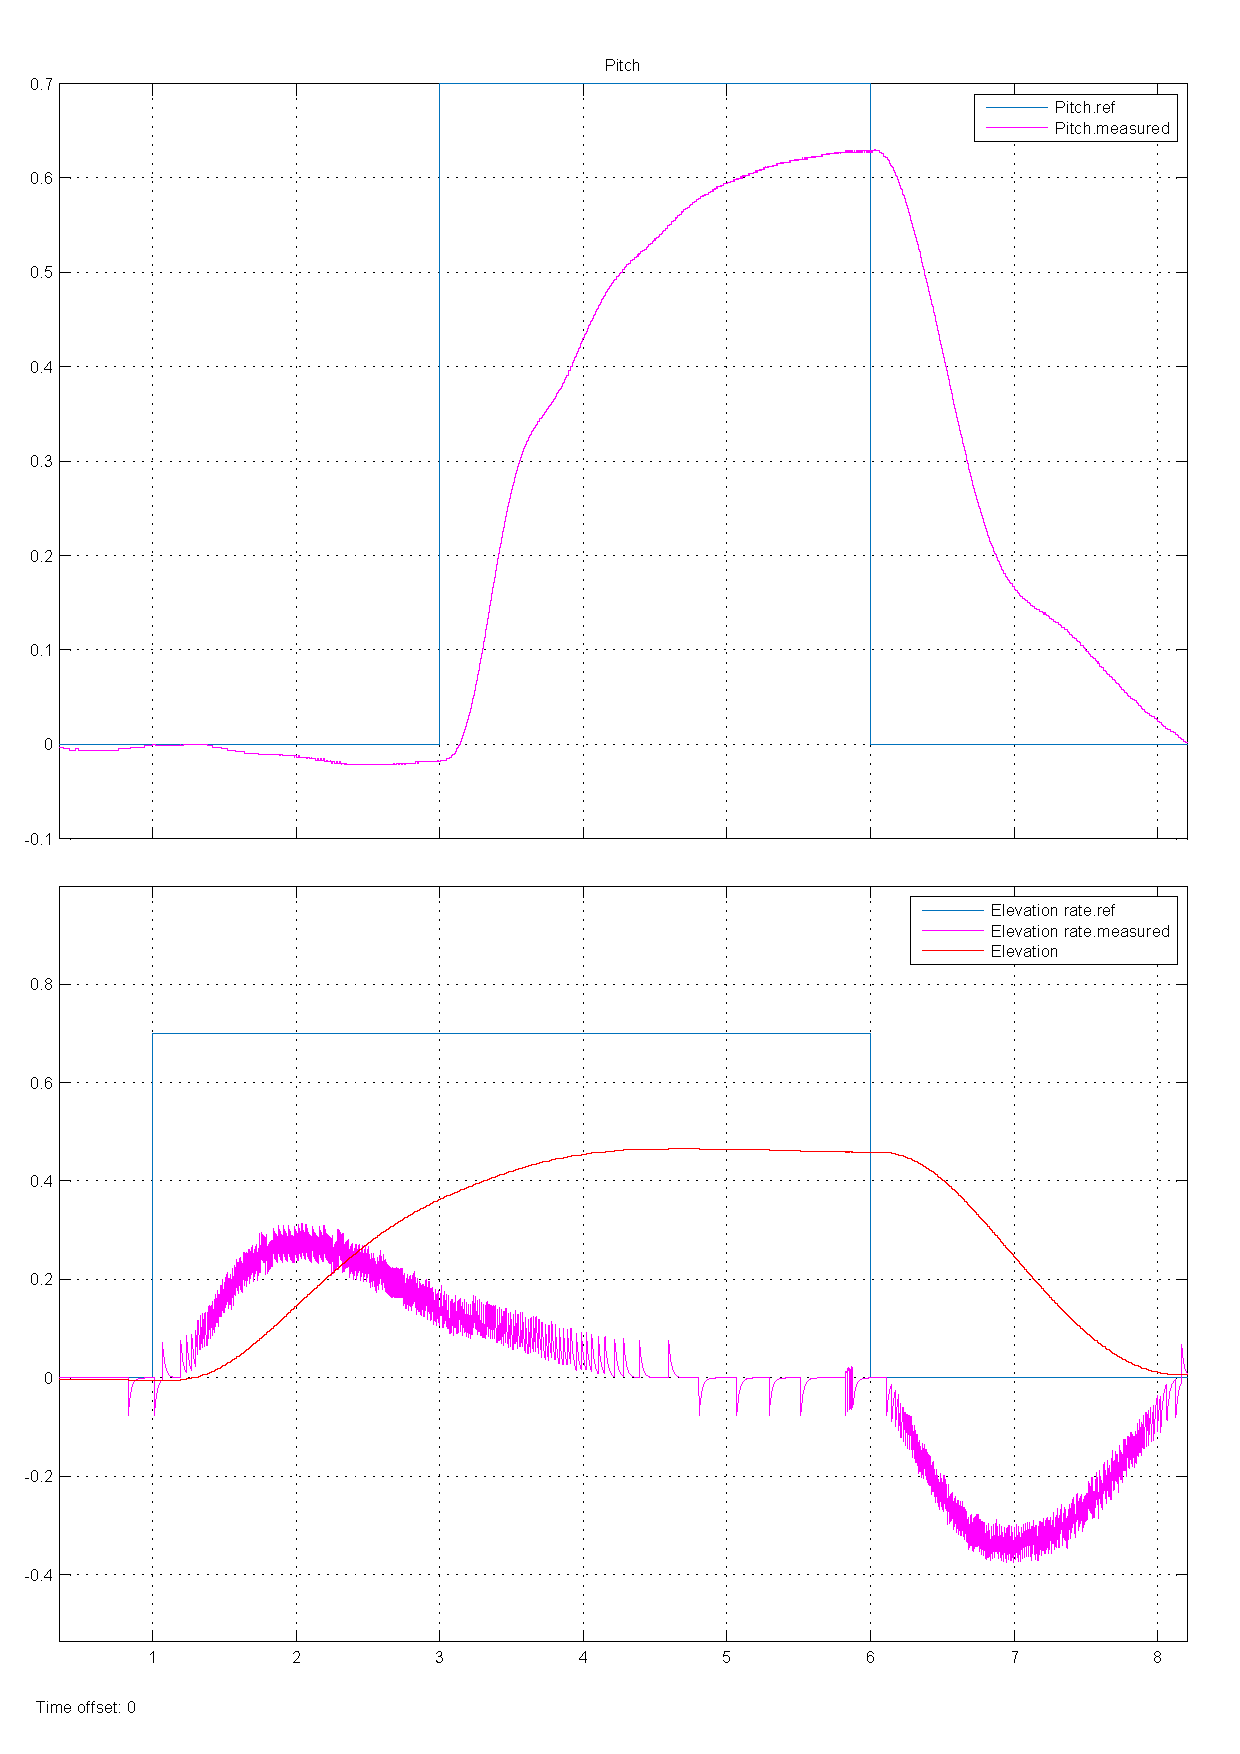
\includegraphics[width=\textwidth]{figures/P3p2_good.pdf}
	\caption{Helicopter response without integral effect, pitch on top and elevation below}
\label{fig:P3p2_plot}
\end{figure}

\begin{figure}[htb]
	\centering
		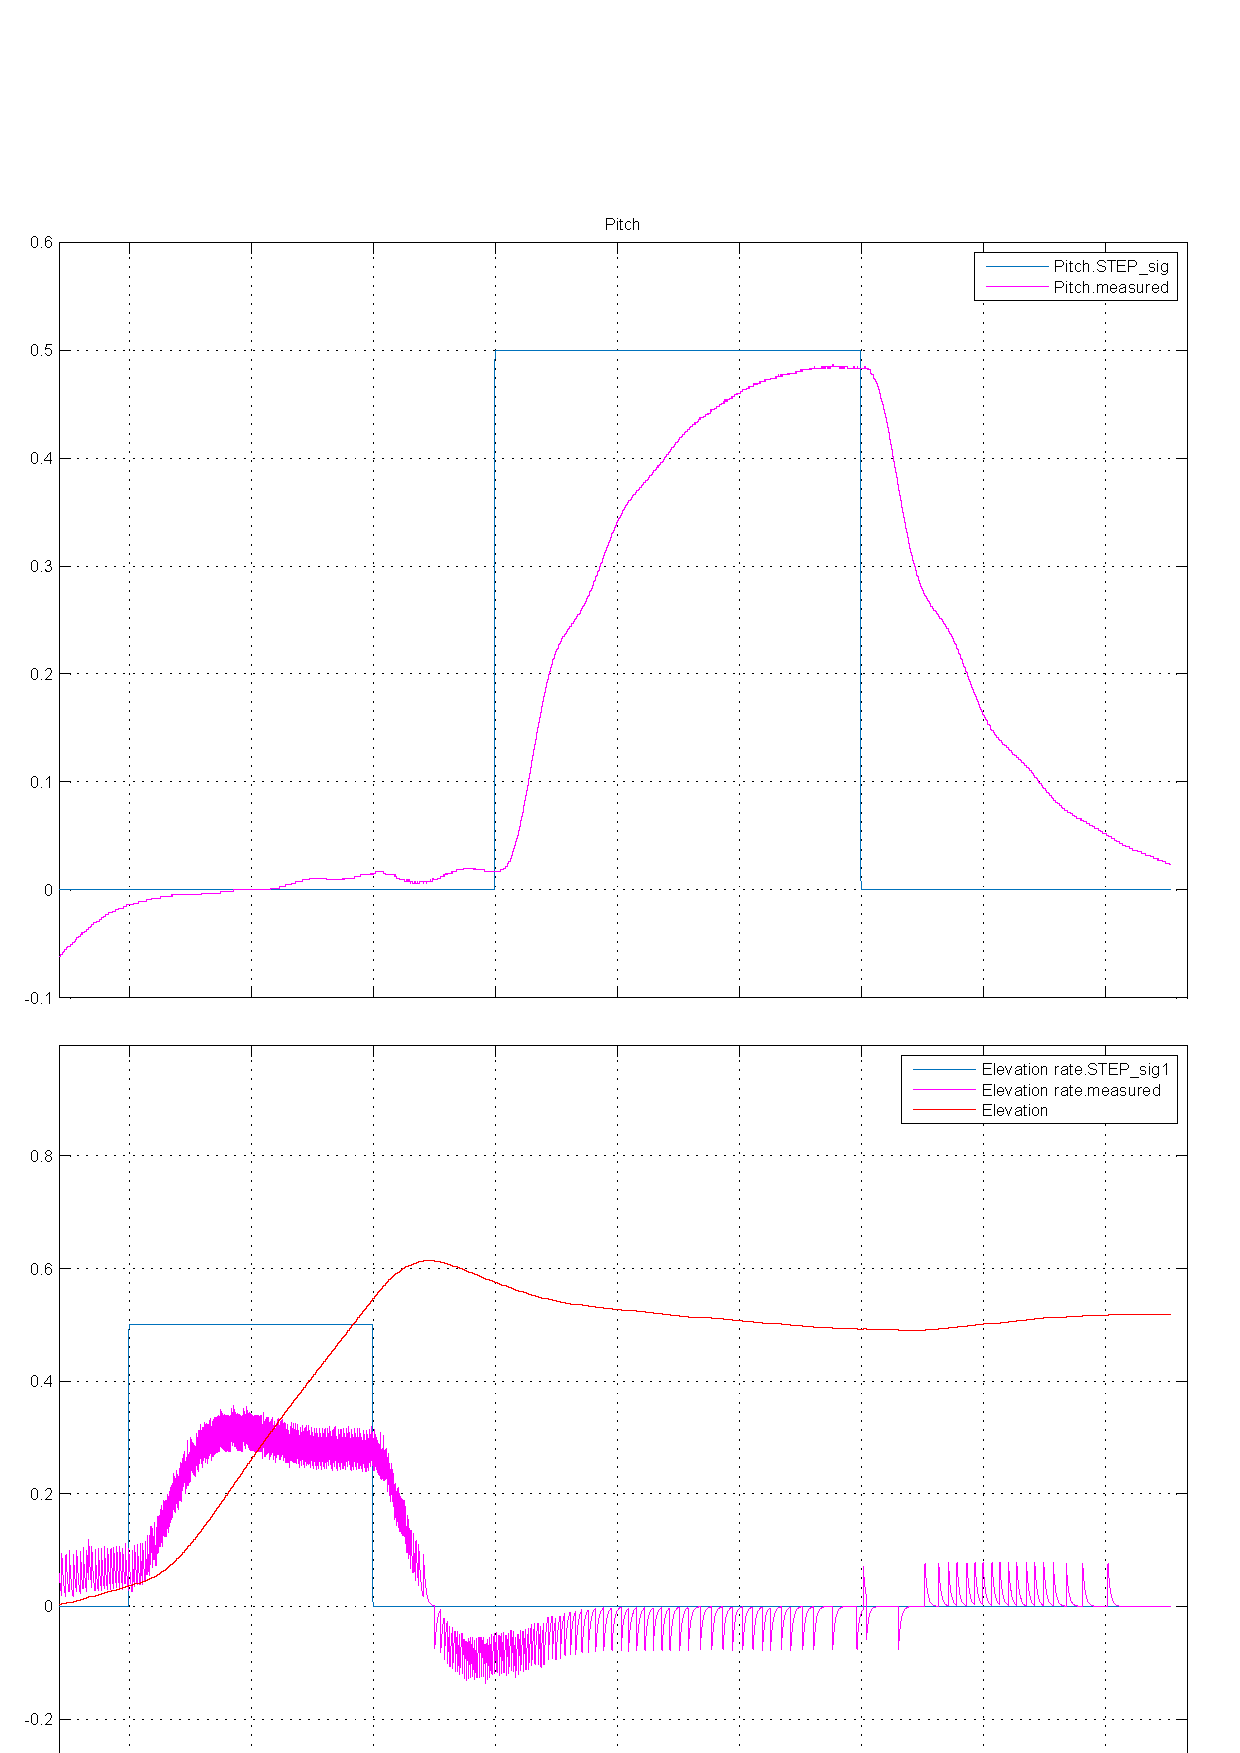
\includegraphics[width=\textwidth]{figures/P3p3_good.pdf}
	\caption{Helicopter response with integral effect, pitch on top and elevation below}
\label{fig:P3p3_plot}
\end{figure}










The Matlab script for this problem can be found in \cref{subsec:P3_init.m}. The Simulink model can be found in \cref{sec:simulink} \cref{fig:P3p3} and \cref{fig:P3p3_PI}.